\section{Einleitung}
	In diesem Versuch wurde die Ablenkung von Elektronen in elektrischen und magnetischen Feldern untersucht.
	Die theoretischen Grundlagen sollten zun"achst mit Messdaten "uber\-pr"uft werden.
	Schlie"slich wurden die Erkenntnisse genutzt, um ein einfaches Oszilloskop zu realisieren und die Feldst"arke des Erdmagnetfeldes zu messen.

\section{Funktionsweise und Theoretische Grundlagen}
	Im Folgenden werden aus den wirkenden Kr"aften die zu "uberpr"ufenden Zusammenh"ange hergeleitet.

	\subsection{Elektrische Kraft}
		Im ersten Versuch betrachtet man ausschlie"slich die elektrische Kraft $\vec{F}_\mathrm{el}$, die auf eine Ladung $q$ im elektrischen Feld $\vec{E}$ wirkt.
		In unserem Versuchsaufbau durchl"auft ein Elektronenstrahl eine Anordnung aus Plattenkondesatoren,
		in denen das elektrische Feld "uberall n"aherungsweise senkrecht auf den Kondensatorplatten steht.

		Die Platten haben die L"ange $p$ und seien im Abstand $d$ angebracht. An ihnen liegt eine Spannung $U_\mathrm{d}$ an.
		Die Ladung der Elektronen betr"agt $e$, ihre Masse $m_e$.

		Die Geschwindigkeit $\vec{v}$ der Teilchen l"asst sich in die Komponenten $v_\mathrm{y}$ und $v_\mathrm{z}$ zerlegen,
		die parallel bzw. orthogonal zum elektrischen Feld $\vec{E}$ stehen.

		Es kann damit eine Aussage "uber den Winkel $\theta$ zwischen $v_\mathrm{y}$ und $v_\mathrm{z}$ getroffen werden:

		\begin{eqnarray}
			\theta & = & \frac{e}{m_e} \frac{U_\mathrm{d}}{d} \frac{p}{v_\mathrm{z}^2}
			\label{theta}
		\end{eqnarray}

		\begin{figure}[h]
			\centering
			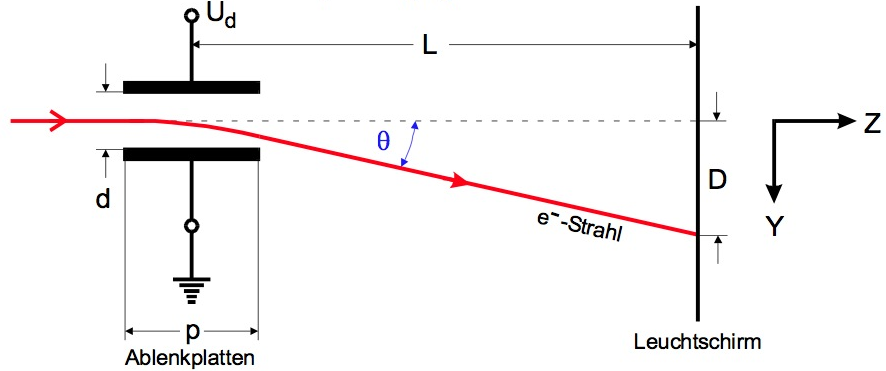
\includegraphics[width = 14cm]{img/ablenkung.png}
			\caption{Strahlablenkung durch einen Plattenkondensator}
			\label{ablenkung}
		\end{figure}

		Unter Ber"ucksichtigung der Beschleunigungsspannung $U_\mathrm{B}$ (siehe \ref{wehnelt}) gilt f"ur die Verschiebung $D$ im Abstand $L$ und parallel zu $\vec{E}$:

		\begin{eqnarray}
			D & = & \frac{p}{2d} L \frac{U_\mathrm{d}}{U_\mathrm{B}}
			\label{verschiebung}
		\end{eqnarray}

		$D$ ist proportional zur Beschleunigungsspannung $U_\mathrm{B}$, kann also zur Spannungsmessung genutzt werden.

	\subsection{Die Braunsche R"ohre}

		Dieser Aufbau ist Teil der \emph{Braunschen R"ohre}. Dieses Ger"at beinhaltet neben den Ab\-lenk\-kon\-den\-sa\-to\-ren, die oben behandelt wurden,
		einen \emph{Wehnelt-Zylinder}, der einen Elektro\-nen\-strahl emittiert,
		eine Vorrichtung, um diesen Strahl zu fokkussieren
		und einen fluoris\-zieren\-den Schirm, der den Aufpunkt des Elektronenstrahles visualisiert.

		Die gesamte R"ohre ist evakuiert, damit die Elektronen nicht mit Luftmolek"ulen zu\-sam\-men\-sto\-"sen und gebremst werden.

		\begin{figure}[h]
			\centering
			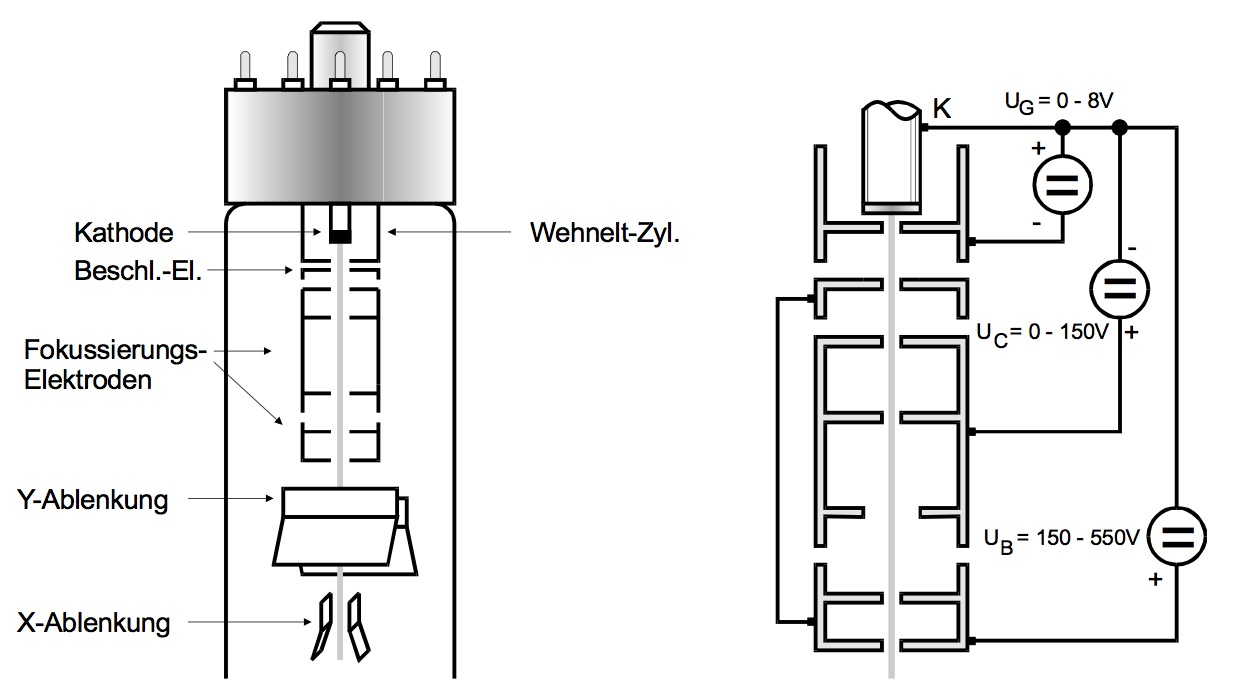
\includegraphics[width = 14cm]{img/wehnelt-z.jpg}
			\caption{Schematischer Aufbau der Braunschen R"ohre -- der Leuchtschirm ist hier nicht sichtbar}
			\label{ablenkung}
		\end{figure}

		\subsubsection{Wehnelt-Zylinder}
		\label{wehnelt}

			Zun"achst wird ein Elektronenstrahl erzeugt. Hierf"ur heizt ein stromdurchflossener Draht einen Zylinder aus einem Material mit geringer Elektronenaustrittsarbeit auf.
			Durch Gl"uhemission treten bei gen"ugend gro"ser Temperatur Elektronen aus.
			Der Zylinder ist von dem gr"o"seren Wehnelt-Zylinder umgeben und es liegt eine Spannung an, sodass der innere Zylinder positiv und der "au"sere negativ geladen ist.
			Durch eine kleine "Offnung in der Stirnseite des Wehnelt-Zylinders treten gerade die Elektronen aus, die gen"ugend kinetische Energie besitzen, um die Potentialbarriere zu "uberwinden.

			Mit einem weiteren Zylinder, der positiv mit der Spannung $U_\mathrm{B}$ geladen ist, werden die Elektronen anschlie"send beschleunigt,
			wobei $v \ll \mathrm{c}$ ist und somit nicht relativistisch gerechnet werden muss.
			Das Durchlaufen dieser Spannung stellt n"aherungsweise die gesamte kinetische Energie f"ur die Elektronen bereit.

		\subsubsection{Fokkusiervorrichtung}

			Die darauffolgende Anordnung aus positiv geladenen Zylindern dient der Fokussierung des Strahls.
			Das elektrische Feld in diesem Bereich wirkt "ahnlich wie Linsen in der Optik.
			Durch Variation der Spannung $U_\mathrm{C}$ kann der Fokus des Strahls ge"andert werden, sodass dieser auf dem Leuchtschirm scharf ist.

		\subsubsection{Ablenkplatten}

			Vor dem Leuchtschirm befinden sich zwei Kondensatoren, deren Platten senkrecht zu\-ein\-ander stehen. Hierdurch kann der Strahl in die Richtungen x und y abgelenkt werden.

			Der Winkel $\theta$, in dem der Kondensator verlassen wird, wird durch Gleichung \ref{theta} be\-schrie\-ben.

			Indem an eine Achse eine S"agezahnspannung mit variabler Frequenz $\omega_\mathrm{takt}$ angelegt wird, kann hiermit ein einfaches Oszilloskop realisiert werden.
			Das Eingangssignal mit fester Frequenz $\omega_\mathrm{sig}$ muss dann an die andere Achse angelegt werden.
			Durch Anpassen der beiden Frequenz $\omega_\mathrm{takt}$ an $\omega_\mathrm{sig}$ l"asst sich ein stehendes Bild des Eingangssignales erzeugen.

		\subsubsection{Leuchtschirm}

			Der Elektronenstrahl trifft schlie"slich auf einen Schirm mit fluoriszierender Beschichtung.
			Die Elektronen wechselwirken mit denen des Schirms und Photonen werden emittiert. Dadurch k"onnen wir den Aufpunkt des Strahls sehen.

	\subsection{Magnetische Kraft (Lorentzkraft)}

		Die magnetische Kraft $\vec{F}_\mathrm{L}$ wirkt nur auf, zum Magnetfeld $\vec{B}$ senkrecht bewegte La\-dun\-gen $q$:

		\begin{eqnarray}
			\vec{F}_\mathrm{L} & = & q \left( \vec{v} \times \vec{B} \right)
		\end{eqnarray}

		Tritt ein Elektron also in ein homogenes Magnetfeld begibt es sich auf eine Kreisbahn.
		Die Lorenztkraft $\vec{F}_\mathrm{L}$ wirkt dann als Zentripetalkraft.

		Ist die St"arke $B$ des Magnetfeldes und die Geschwindigkeit $v_0$ des Elektrons bekannt, l"asst sich der Radius $r$ seiner Kreisbahn messen und es gilt:

		\begin{equation}
			r = \frac{m_e}{e} \frac{v_0}{B}
		\end{equation}
	
		Damit kann man also die spezifische Ladung $e / m_e$ bestimmen.\\

		Durch eine Helmholtz-Spule l"asst sich ein nahezu homogenes Magnetfeld erzeugen.
		Setzt man nun eine Braunsche R"ohre in dieses Magnetfeld l"asst sich der folgende Aufbau gut realisieren.

		\begin{figure}[h]
			\centering
			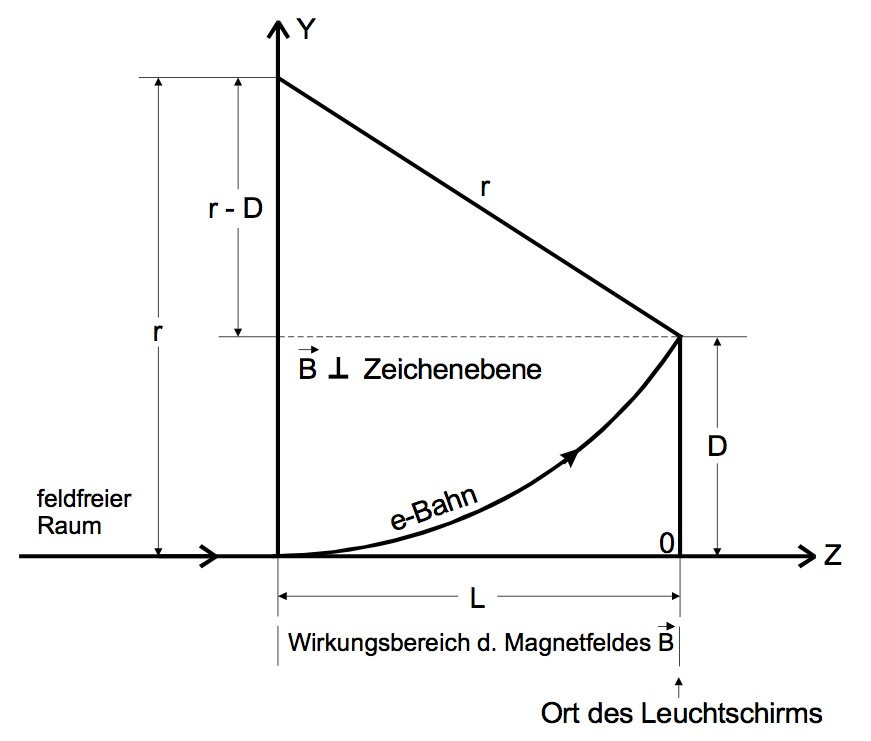
\includegraphics[width = 12cm]{img/magnetfeld.jpg}
			\caption{Strahlablenkung in einem Magnetfeld}
			\label{magnetfeld}
		\end{figure}

		Die Wegl"ange der Elektronen innerhalb der Ablenkkondensatoren der Braunschen R"ohre kann dabei vernachl"assigt werden.
		Die Strecke $L$ ist somit der Weg zwischen Ab\-lenk\-plat\-ten und Leuchtschirm.
		Das Magnetfeld $B$ ist proportional zum Strom $I$ durch die Helm\-holtz\-spu\-le.
		Es gilt dann:

		\begin{equation}
			\sqrt{\frac{e}{m_e}} = \frac{\sqrt{8 U_\mathrm{B}}}{B} \frac{D}{L^2 + D^2}
		\end{equation}
